\chapter{Prezentarea aplica\c tiei}

Aplicația ManFast rulează în browser la \texttt{http://localhost:5173} (frontend) și comunică cu API-ul Express la portul 5000. În acest capitol sunt ilustrate interfețele principale.

\section{Utilizarea aplicației — perspectiva utilizatorului}

\subsection{Pagina principală}

Pagina principală afișează evenimentele viitoare sub formă de listă orizontală. Componenta \texttt{EventSearchFilters} permite filtrarea după nume, județ (select din 42 județe) și dată. Evenimentele expirate (data + durata) nu apar în listă.

Utilizatorul neautentificat poate naviga și filtra evenimente. Pentru cumpărare bilet este necesară autentificarea. Designul folosește carduri \texttt{EventListItem} cu titlu, locație, preț și locuri disponibile. Navbar-ul conține link-uri către ,,Evenimente``, ,,Biletele mele`` și ,,Profil`` (vizibile doar autentificat), plus buton ,,Panou Admin`` pentru rol admin.

Filtrarea pe județ utilizează lista completă județelor din \texttt{constants/judete.js}, aliniată la organizarea administrativă din România. Filtrul pe dată permite restrângerea rezultatelor la o zi specifică, util în planificarea participării la competiții.

\begin{figure}[htbp]
	\centering
	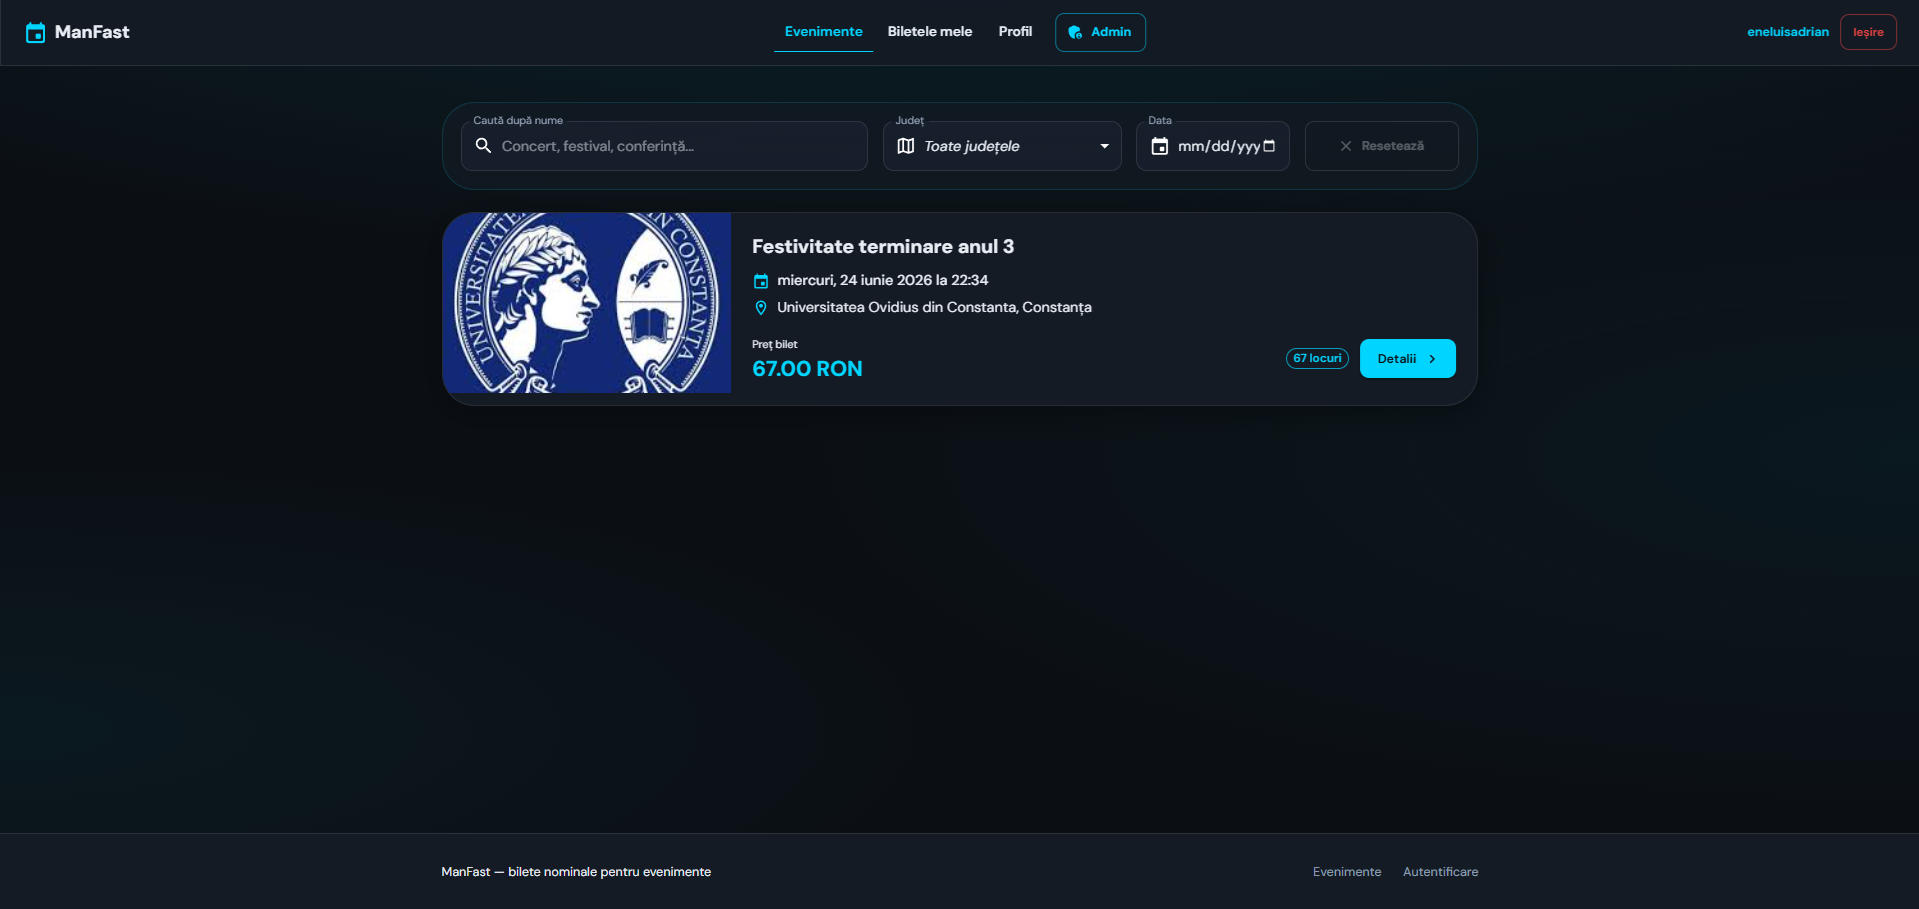
\includegraphics[width=1\textwidth]{paginaprincipala.png}
	\caption{Pagina principală — listă evenimente și filtre}
	\label{fig:l2f1}
\end{figure}



\subsection{Detalii eveniment}

Pagina \texttt{/events/:id} prezintă titlul, galeria de imagini, descrierea, data, județul, localitatea, locația, prețul și locurile disponibile. Utilizatorul autentificat poate adăuga unul sau mai multe câmpuri ,,Nume participant`` și iniția plata Stripe.

Galeria de imagini suportă mai multe fișiere încărcate de admin (max 8, 5MB/fișier). Layout-ul este responsive: pe desktop, detaliile și formularul de cumpărare pot apărea în coloane; pe mobil, stivă verticală. Validarea frontend verifică că toate numele sunt completate înainte de apelul API. La succes, utilizatorul este redirectat către Stripe Checkout hosted page — datele cardului nu tranzitează serverul ManFast.



\begin{figure}[htbp]
	\centering
	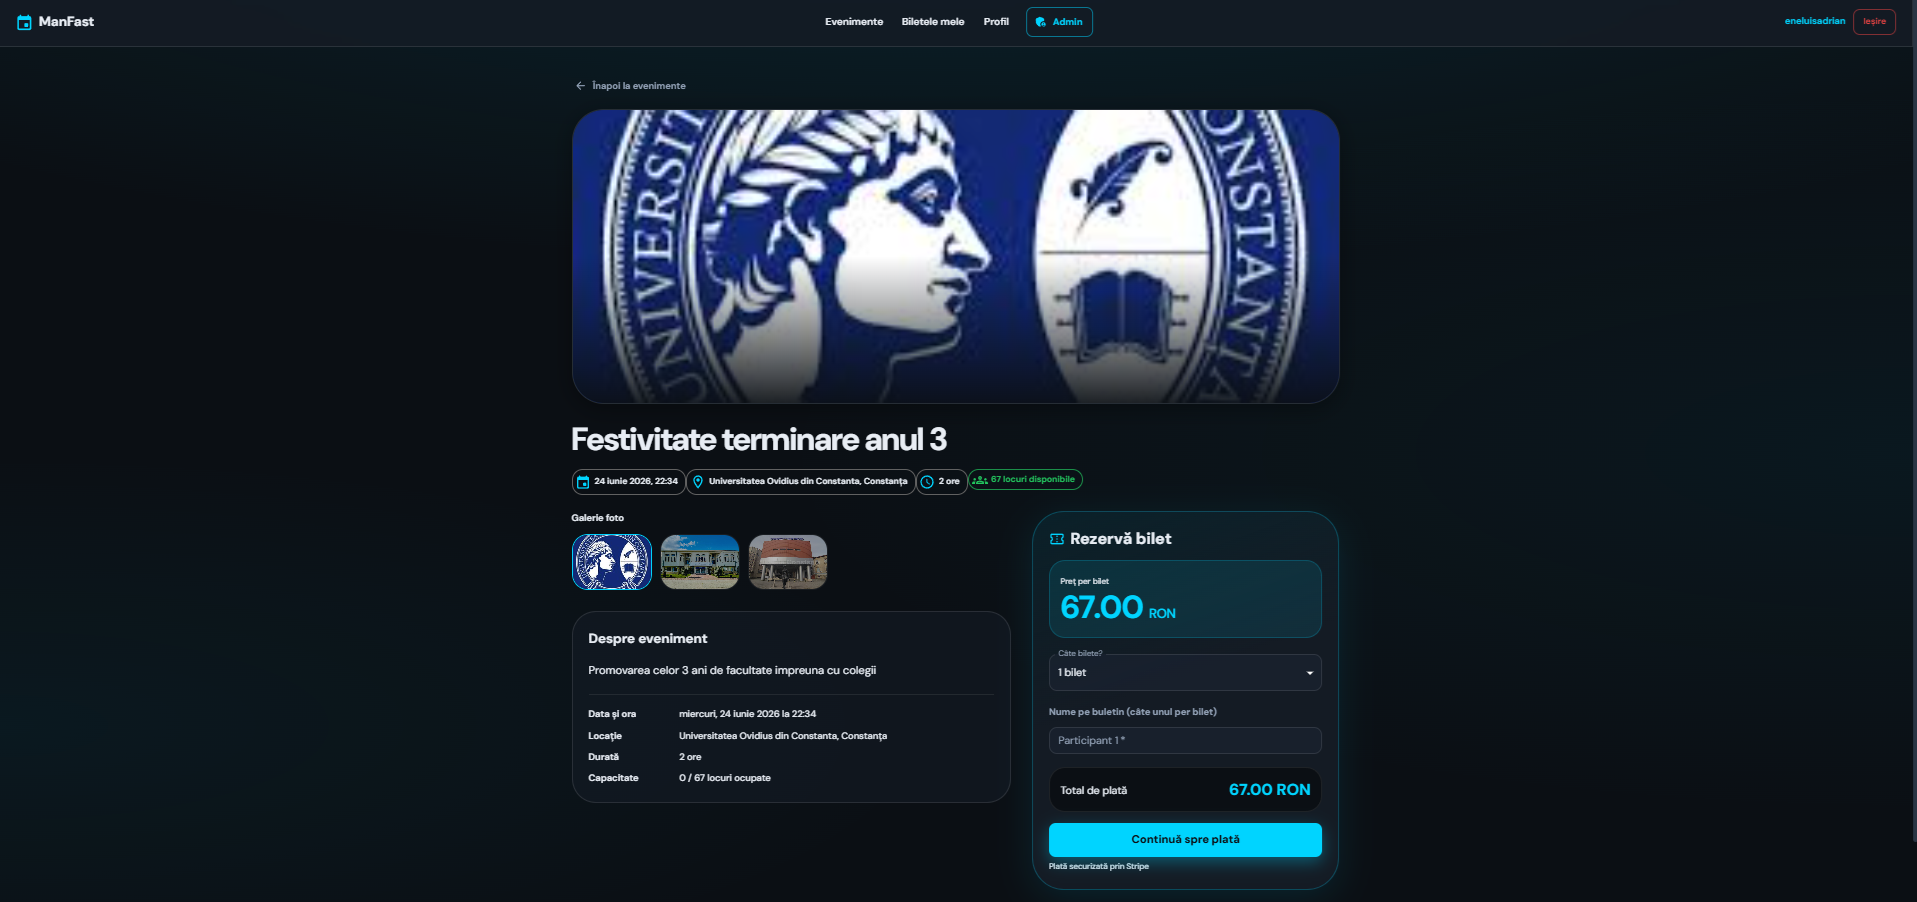
\includegraphics[width=1\textwidth]{Pagina_detalii_eveniment_si_formular_bilete.png}
	\caption{Pagina detalii eveniment și formular bilete}
	\label{fig:l2f1}
\end{figure}

\subsection{Înregistrare cont — pasul 1}

Formularul de înregistrare colectează username, email, telefon, parolă. La submit se apelează \texttt{POST /api/auth/register} și se trece la ecranul de verificare.

\begin{figure}[htbp]
	\centering
	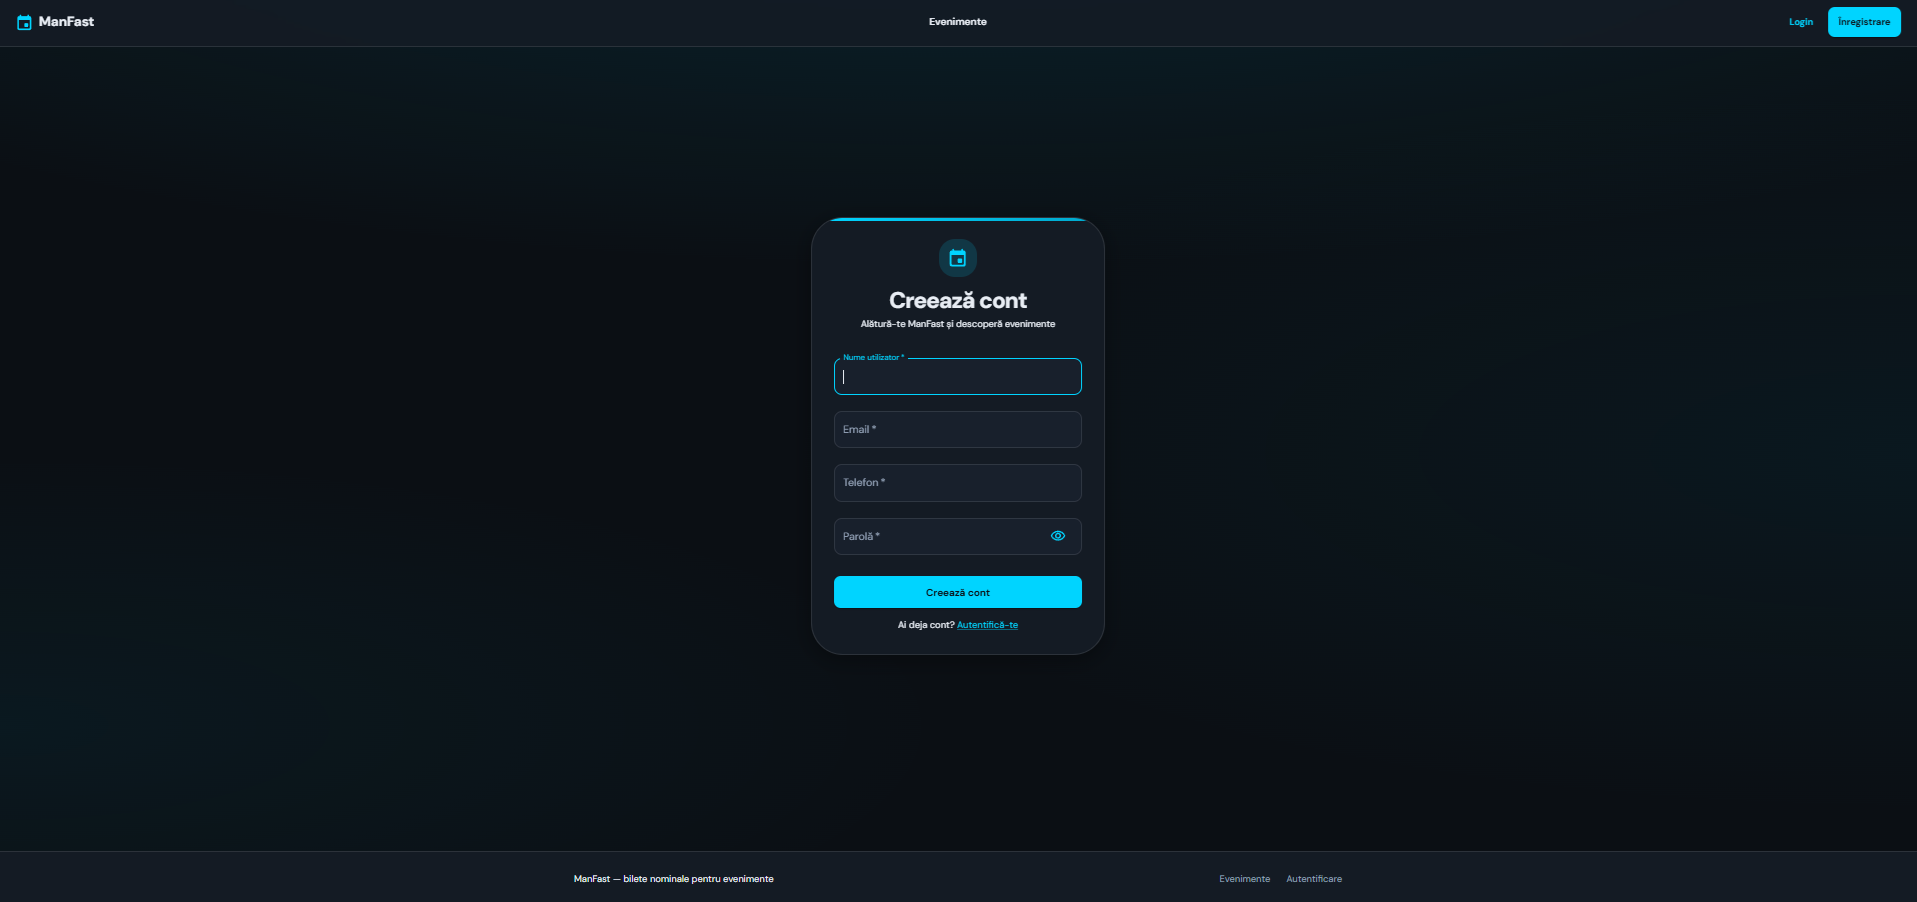
\includegraphics[width=1\textwidth]{Formular_inregistrare.png}
	\caption{Formular inregistrare}
	\label{fig:l2f1}
\end{figure}

\subsection{Verificare email — pasul 2}

Utilizatorul introduce codul de 6 cifre primit pe email. Opțiuni: retrimite cod, înapoi la formular.

\begin{figure}[htbp]
	\centering
	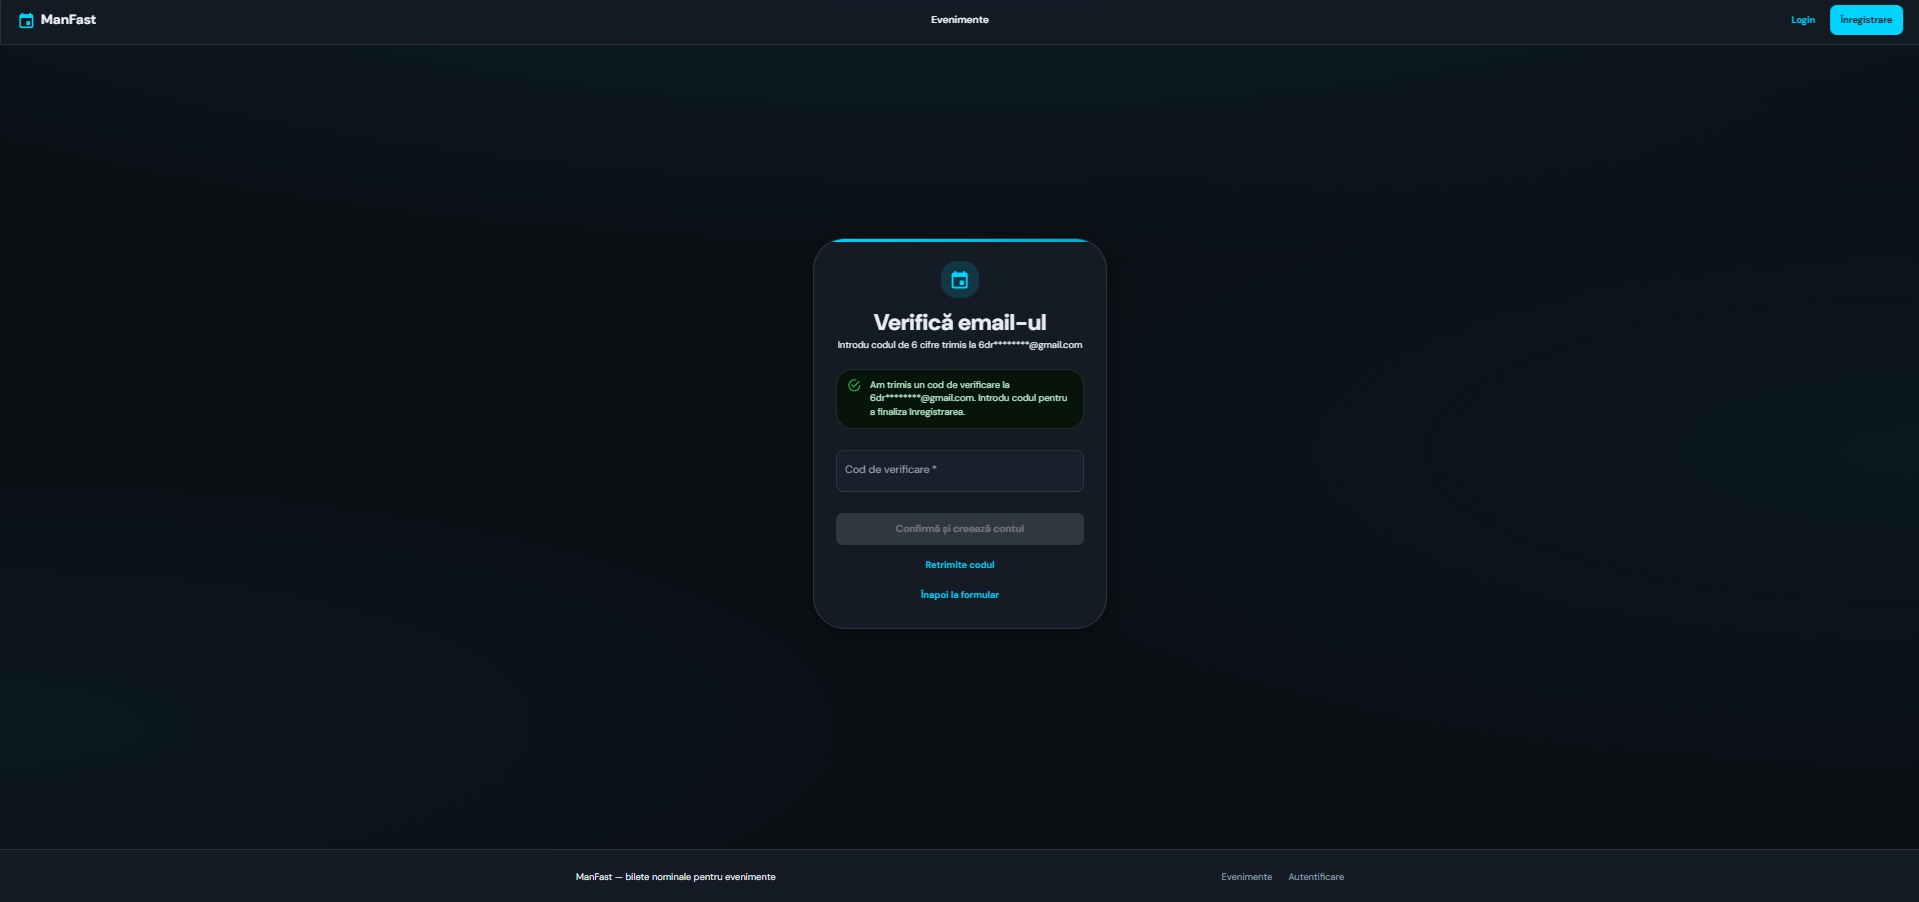
\includegraphics[width=1\textwidth]{Verificare email cu_cod.png}
	\caption{Verificare email cu cod}
	\label{fig:l2f1}
\end{figure}

\subsection{Autentificare}

Pagina \texttt{/login} permite autentificarea. Link-uri către ,,Am uitat parola`` și ,,Înregistrează-te`` (transfer email/parolă prin state).

\begin{figure}[htbp]
	\centering
	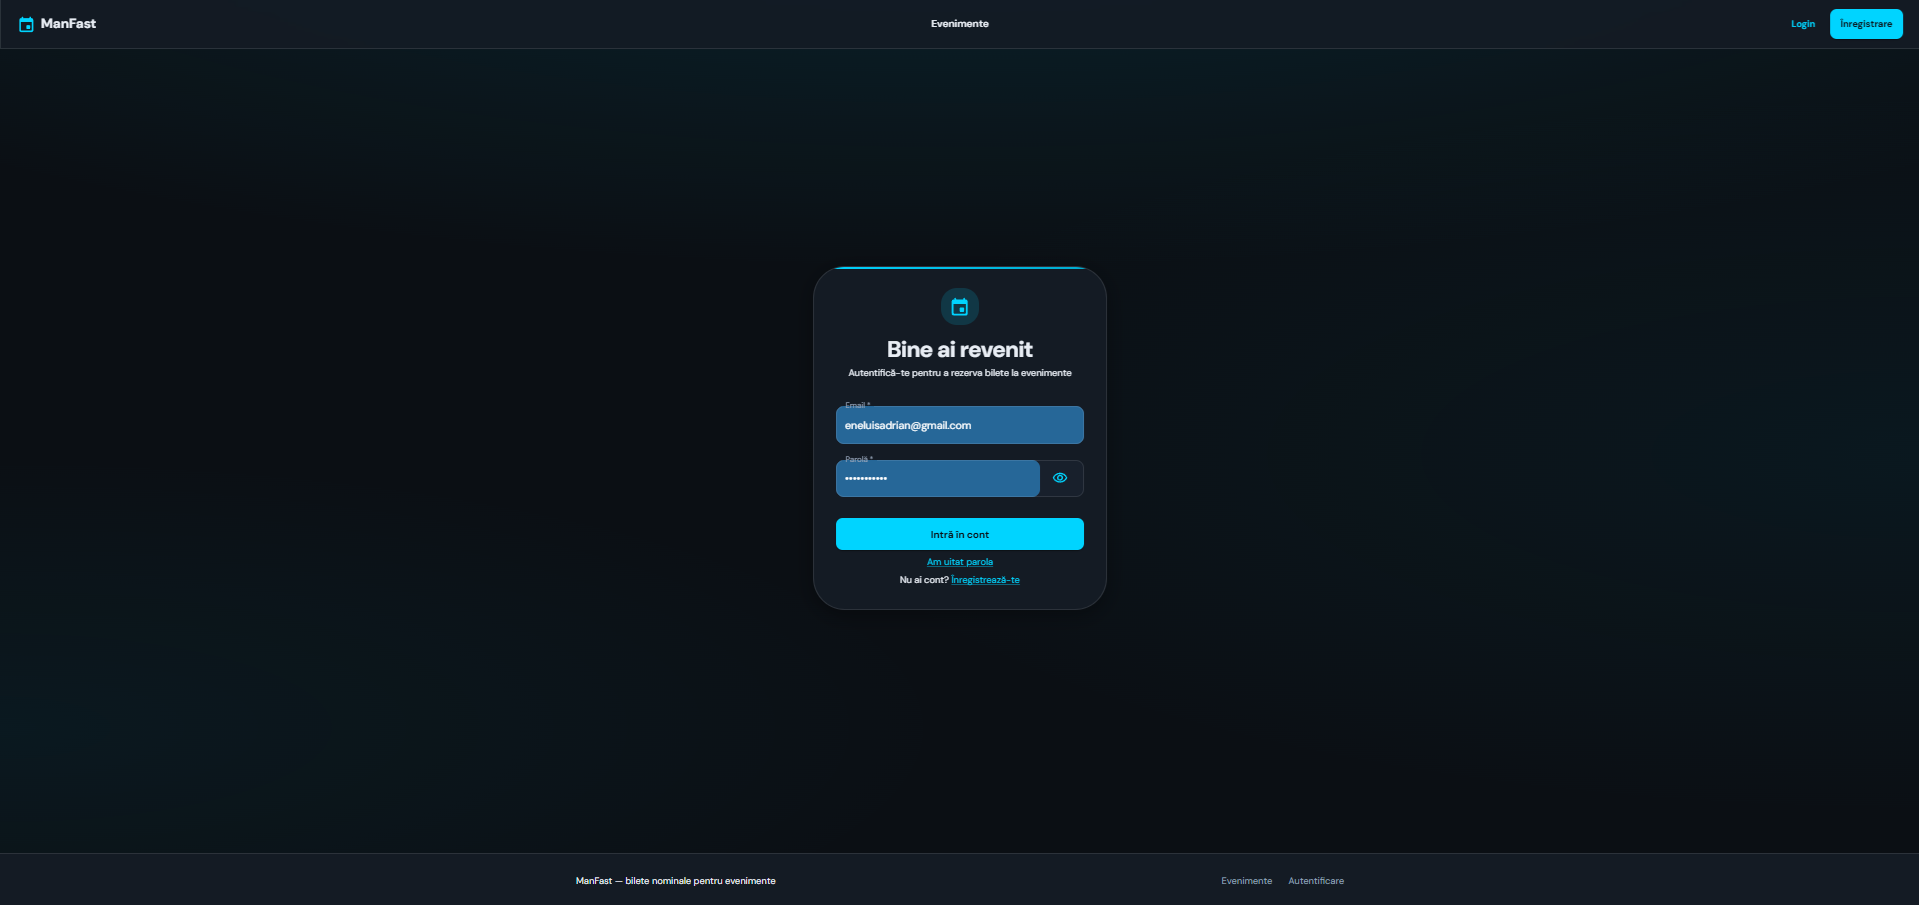
\includegraphics[width=1\textwidth]{Pagina login.png}
	\caption{Pagina login}
	\label{fig:l2f1}
\end{figure}

\subsection{Confirmare plată}

După Stripe Checkout, utilizatorul revine la \texttt{/payment-success?session\_id=...}. Frontend confirmă plata și redirecționează spre bilete.

\begin{figure}[htbp]
	\centering
	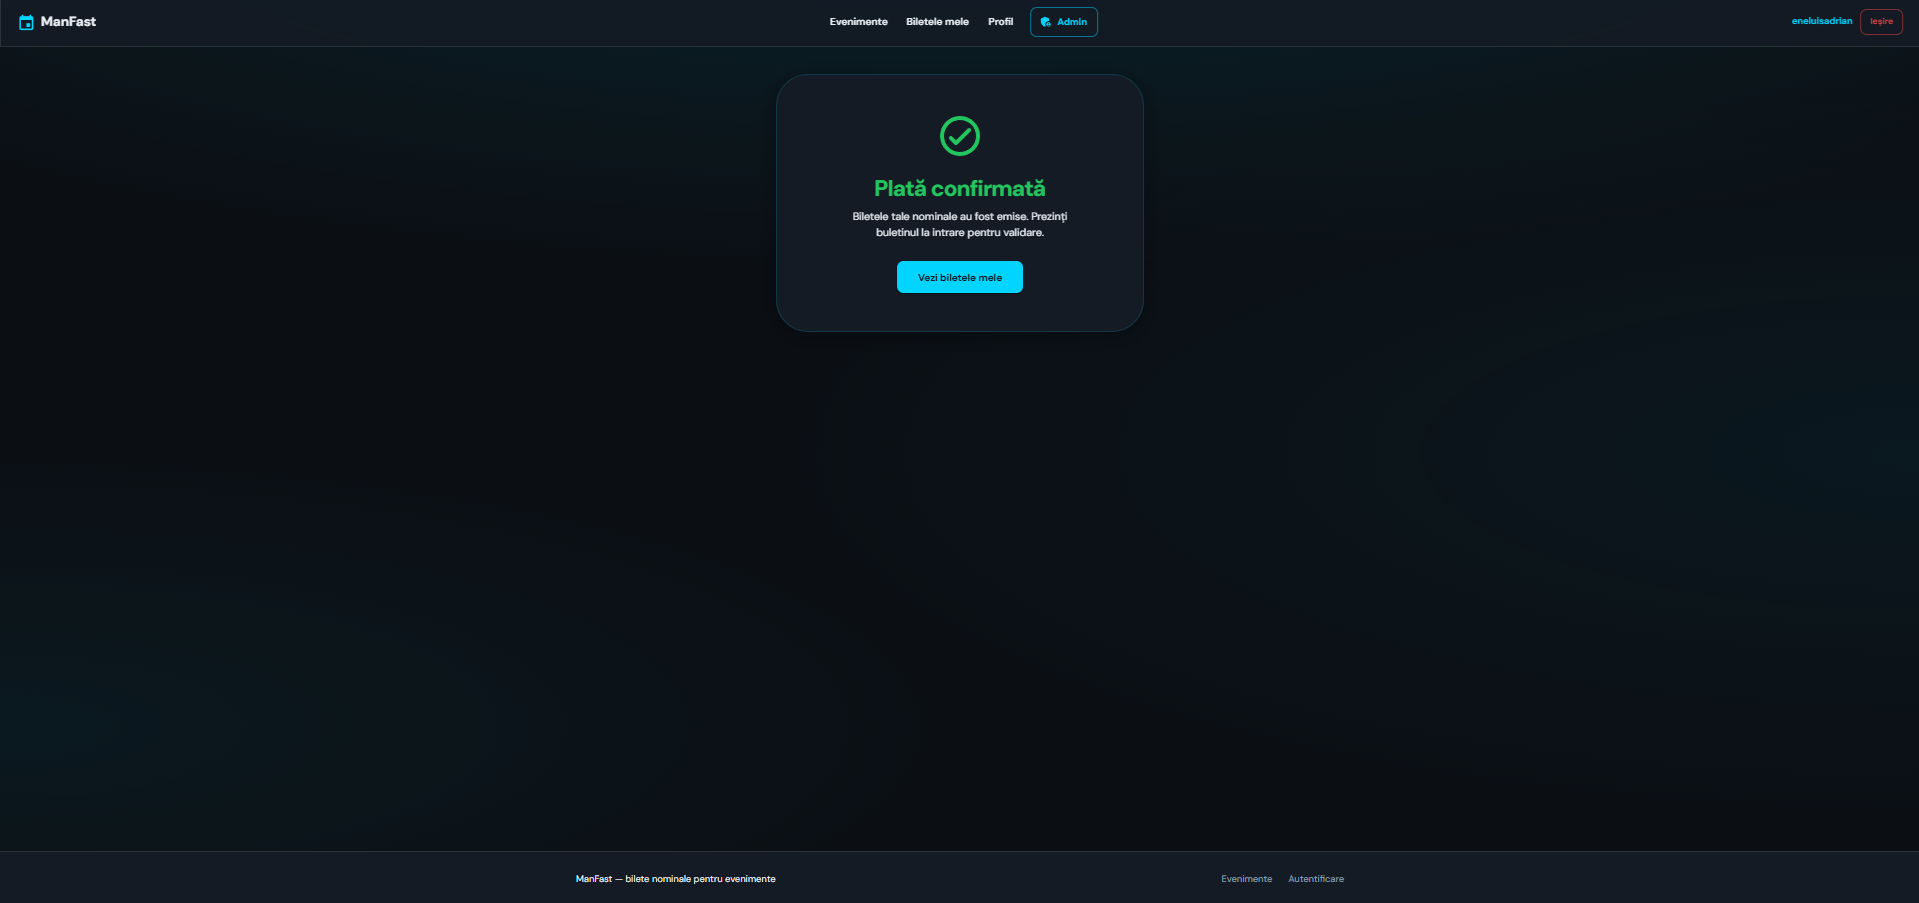
\includegraphics[width=1\textwidth]{Pagina succes plat ˘ a.png}
	\caption{Pagina succesc plata}
	\label{fig:l2f1}
\end{figure}

\subsection{Biletele mele}

\texttt{/my-tickets} grupează biletele în ,,viitoare`` și ,,trecute``. Fiecare card arată evenimentul, numele de pe bilet, status (Plătit / Check-in / Expirat).

\begin{figure}[htbp]
	\centering
	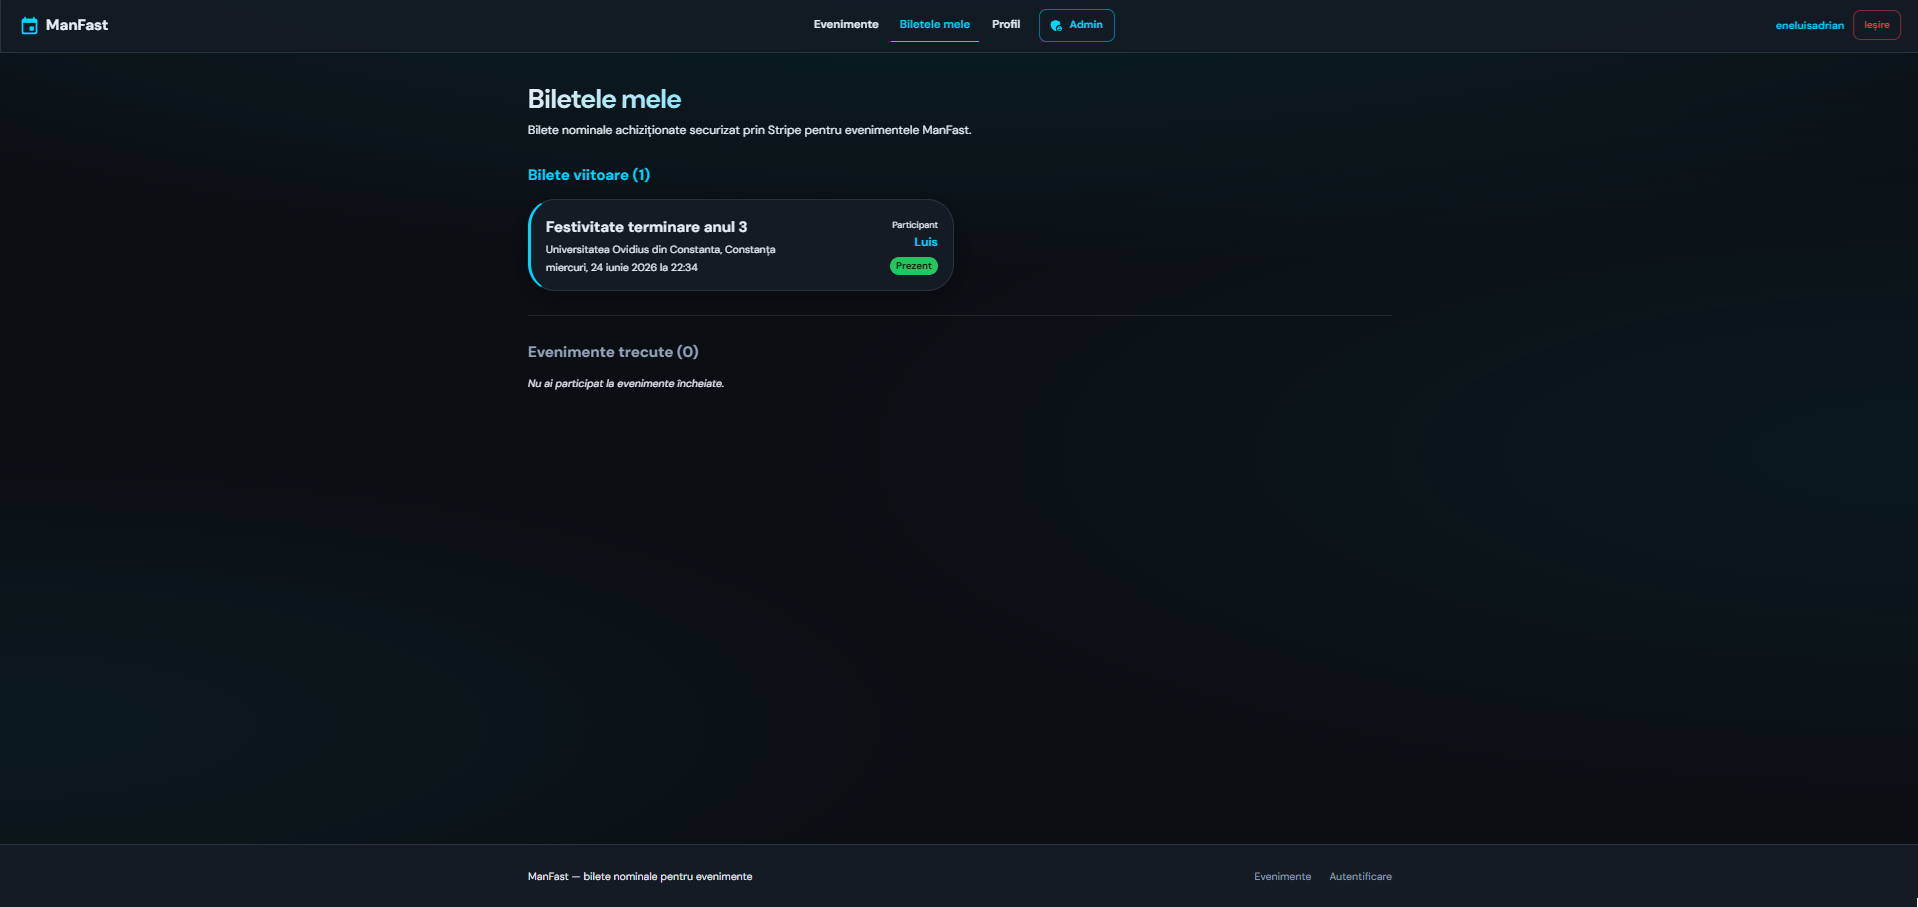
\includegraphics[width=1\textwidth]{Biletele mele.png}
	\caption{Biletele mele}
	\label{fig:l2f1}
\end{figure}

\subsection{Profil utilizator}

\texttt{/profile}: mod vizualizare și mod editare; schimbare parolă; zonă roșie ștergere cont.

\begin{figure}[htbp]
	\centering
	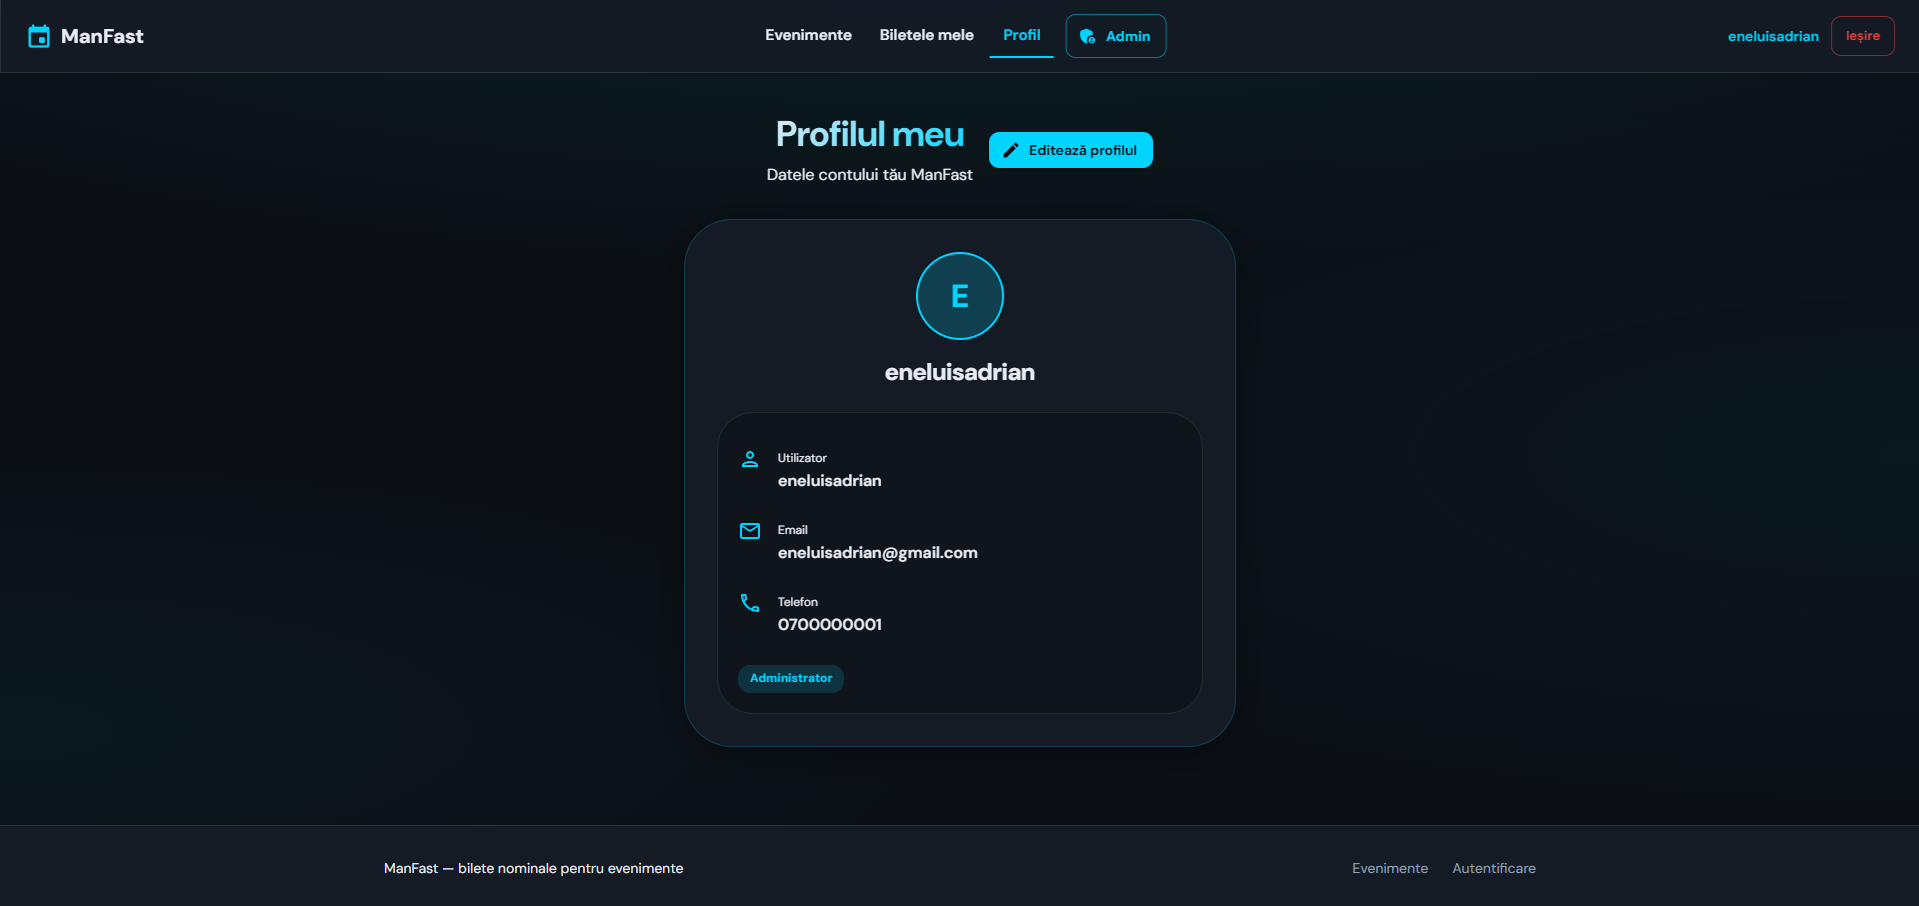
\includegraphics[width=1\textwidth]{Profil utilizator.png}
	\caption{Profil utilizator}
	\label{fig:l2f1}
\end{figure}

\subsection{Resetare parolă — pasul 1 (opțional)}

Formularul ,,Am uitat parola`` acceptă email sau telefon; backend-ul trimite link de reset pe email (mesaj generic pentru confidențialitate).

\begin{figure}[htbp]
	\centering
	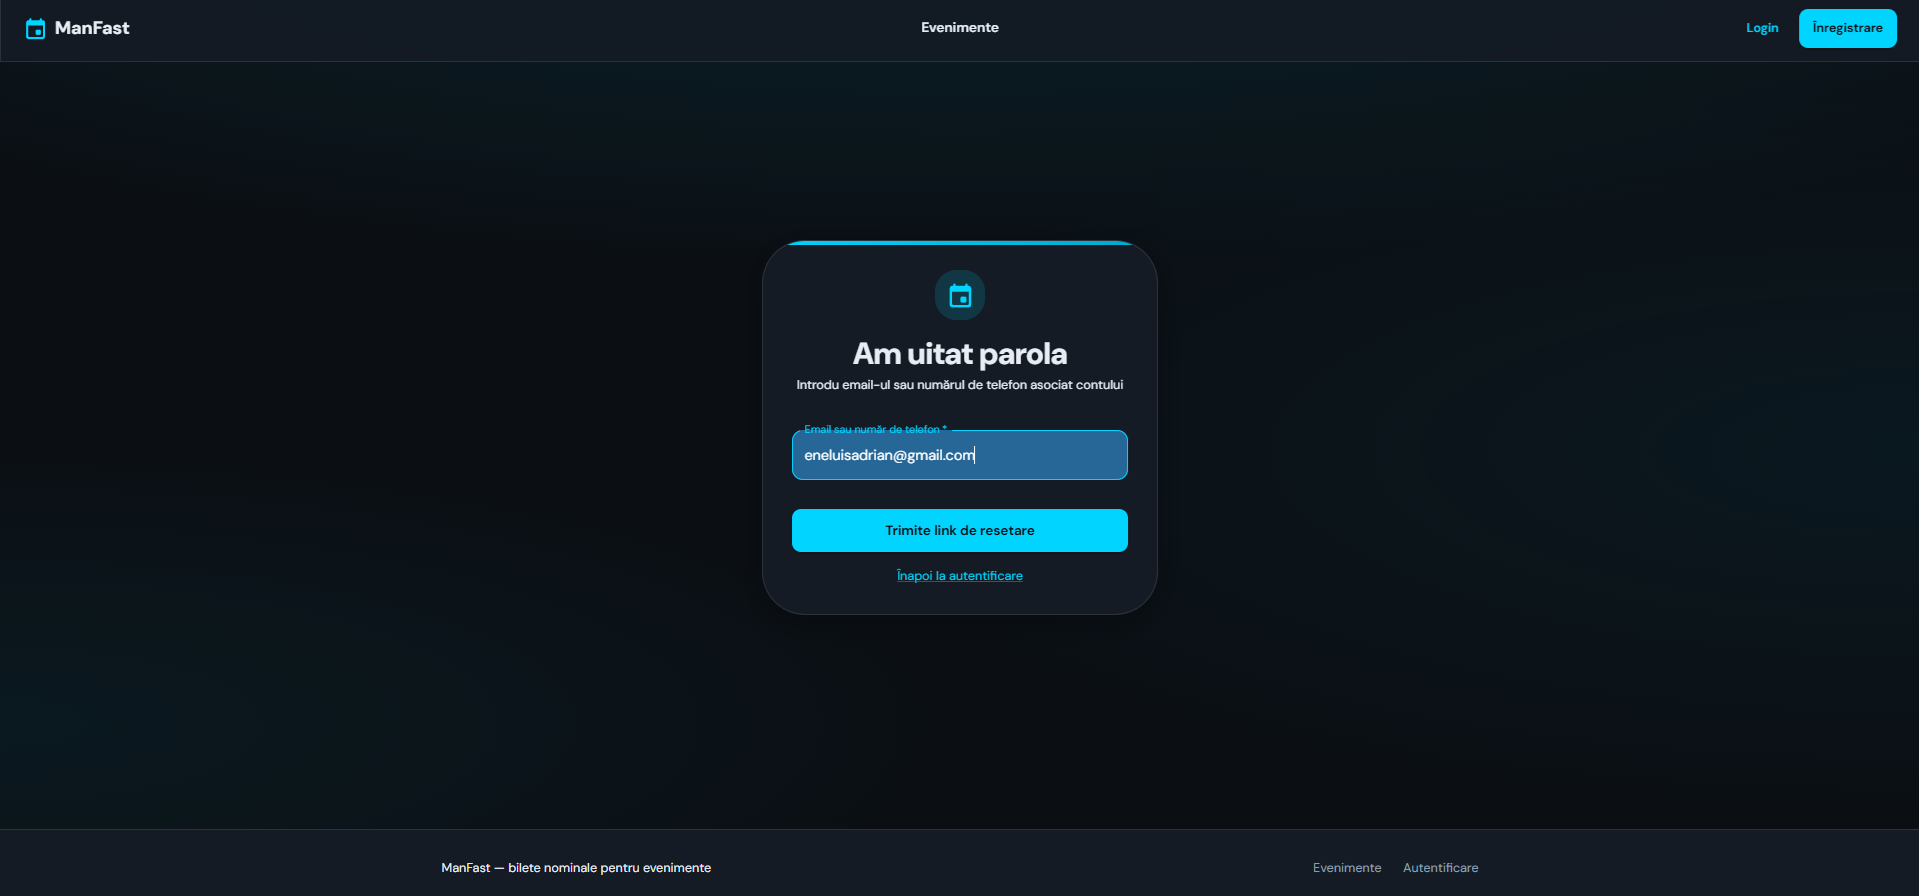
\includegraphics[width=1\textwidth]{Pagina Am uitat parola (opt¸ional).png}
	\caption{Pagina Am uitat parola (opt¸ional)}
	\label{fig:l2f1}
\end{figure}

\subsection{Resetare parolă — pasul 2 (opțional)}

După solicitarea resetării, utilizatorul accesează link-ul din email (\texttt{/reset-password?token=...}) și setează parola nouă. Token-ul este validat server-side (hash SHA-256, expirare 1h).

\begin{figure}[htbp]
	\centering
	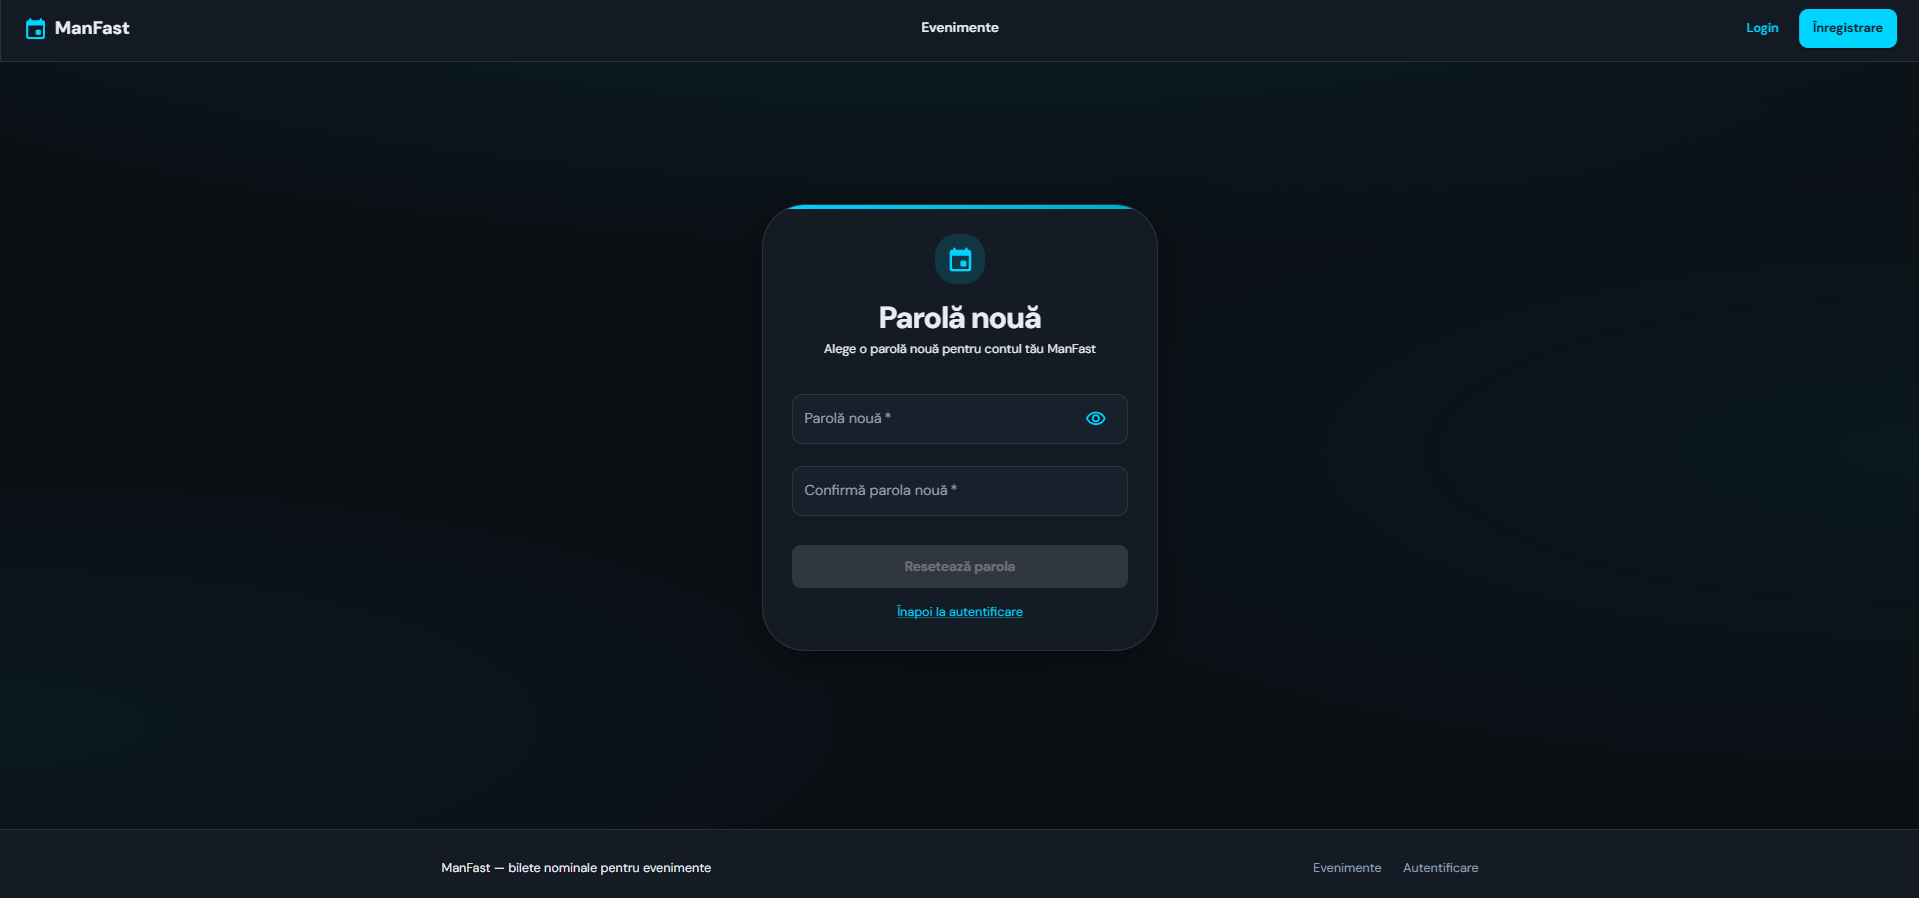
\includegraphics[width=1\textwidth]{Formular parola nou ˘ a (reset).png}
	\caption{Formular parola noua (reset)}
	\label{fig:l2f1}
\end{figure}


\section{Experiență utilizatorului și design responsive}

\subsection{Parcursul utilizatorului (user journey)}

Fluxul complet al unui participant nou poate fi rezumat astfel: descoperire eveniment pe Home $\rightarrow$ consultare detalii $\rightarrow$ redirect la Login/Register dacă nu este autentificat $\rightarrow$ înregistrare cu verificare email $\rightarrow$ revenire la eveniment $\rightarrow$ completare nume participanți $\rightarrow$ plată Stripe $\rightarrow$ confirmare $\rightarrow$ vizualizare bilet in Biletele mele $\rightarrow$ prezentare la check-in (validat de admin)

Fiecare pas este marcat de feedback vizual: stări de încărcare (\texttt{CircularProgress}), mesaje de eroare contextualizate, redirect automat după acțiuni reușite. Transferul email/parolă de la Login la Register (via \texttt{location.state}) reduce fricțiunea pentru utilizatorii care încep de pe pagina greșită.

\subsection{Adaptare mobil și accesibilitate}

Material UI 9 oferă componente responsive (\texttt{Grid}, \texttt{Stack}, \texttt{useMediaQuery}). Navbar-ul comută la meniul hamburger pe ecrane înguste; filtrele pe Home se stivează vertical. Formularele de autentificare sunt centrate în \texttt{AuthCard} cu lățime maximă, ușor de utilizat pe telefon.

Au fost remediate probleme de accesibilitate: focus corect după închiderea meniului mobil (evitare \texttt{aria-hidden} pe elemente focusabile), utilizarea etichetelor \texttt{label} pe câmpuri, contrast ridicat în tema dark (cyan pe fundal întunecat).

\subsection{Mesaje de eroare și stări goale}

Listele goale (fără evenimente, fără bilete) afișează text explicativ și sugestii (ex. ,,Modifică filtrele`` sau ,,Cumpără primul bilet``). Erorile API (429 rate limit, 401 sesiune expirată) sunt traduse în mesaje inteligibile, fără detalii tehnice expuse utilizatorului final.

\section{Utilizarea aplicației — perspectiva administratorului}

Administratorul accesează \texttt{/admin} după autentificare cu rol \texttt{admin}. Componenta \texttt{AdminRoute} verifică token JWT și rol; utilizatorii obișnuiți sunt redirecționați.

Panoul centralizează gestionarea evenimentelor și a participanților. Administratorul poate crea evenimente noi, edita pe cele existente (inclusiv adăugare imagini incremental), șterge evenimente (cu confirmare dialog) și vizualiza participanți cu status check-in. Gestionarea administratorilor se face într-un dialog separat, protejat de parolă de autorizare configurată în \texttt{.env}.

\subsection{Panou admin — dashboard}

Listă evenimente cu acțiuni editare/ștergere; tab participanți; check-in.

\begin{figure}[htbp]
	\centering
	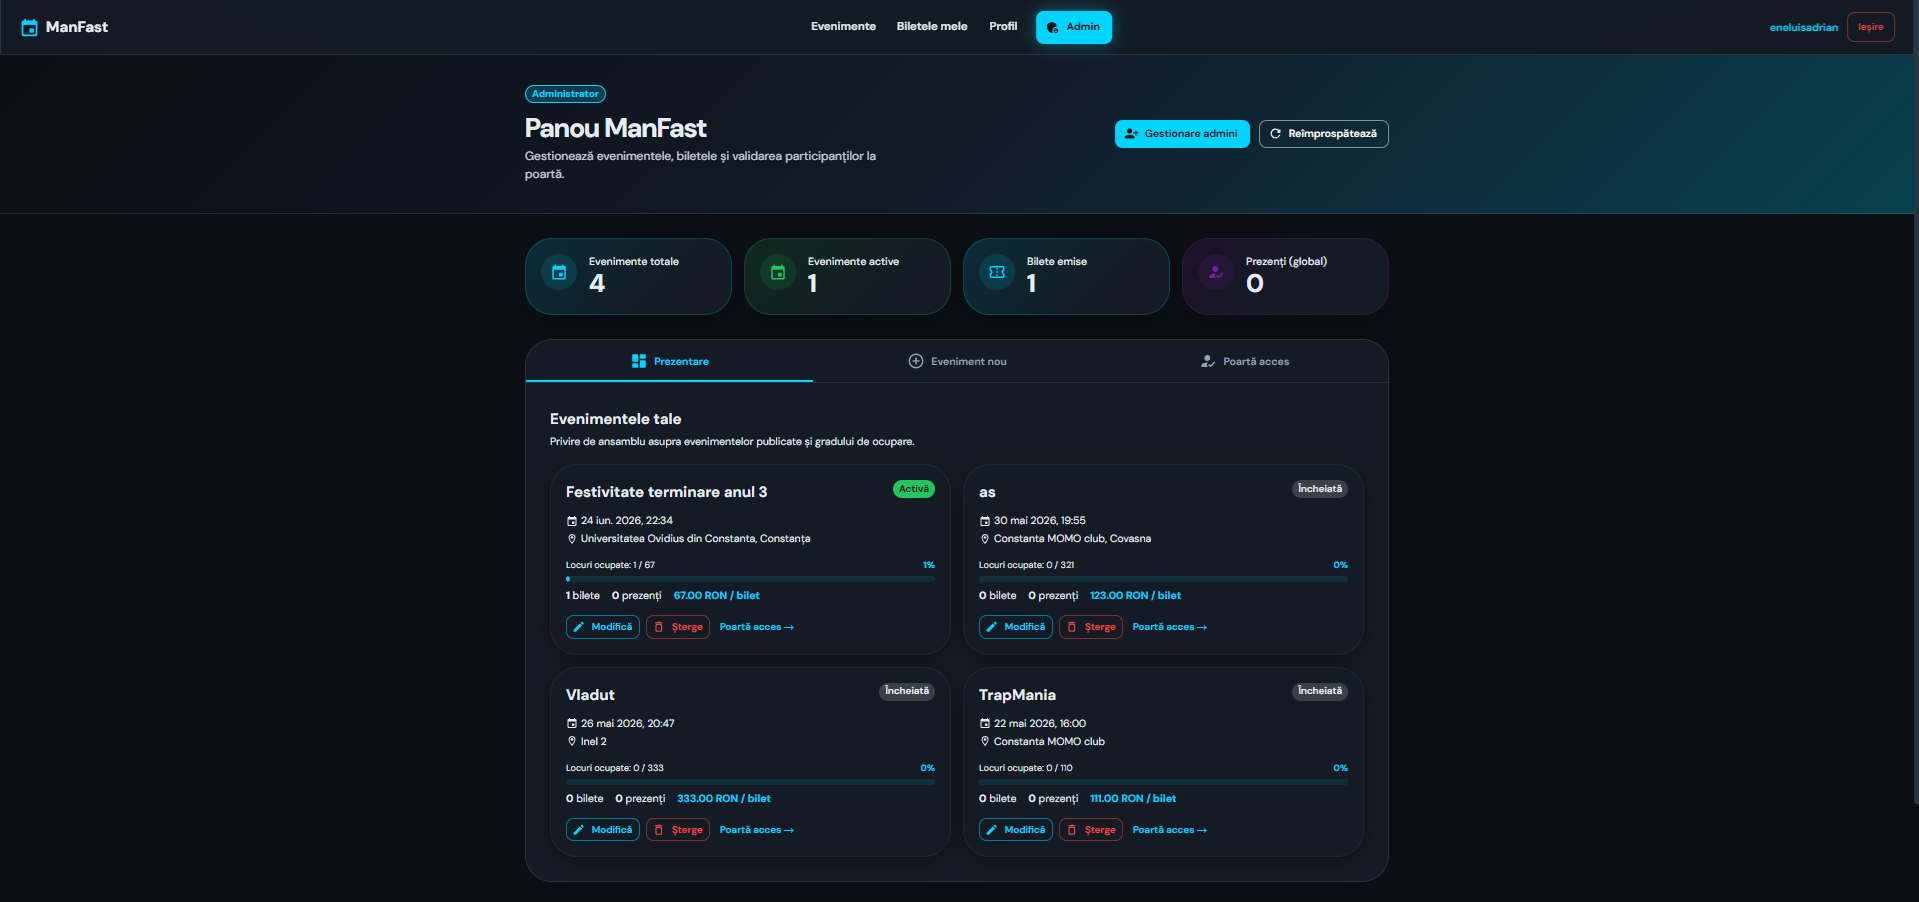
\includegraphics[width=1\textwidth]{Panou admin — dashboard.png}
	\caption{Panou admin — dashboard}
	\label{fig:l2f1}
\end{figure}

\subsection{Creare / editare eveniment}

Dialog cu câmpuri: titlu, descriere, dată, județ, localitate, preț, locuri, durată, upload imagini.

\begin{figure}[htbp]
	\centering
	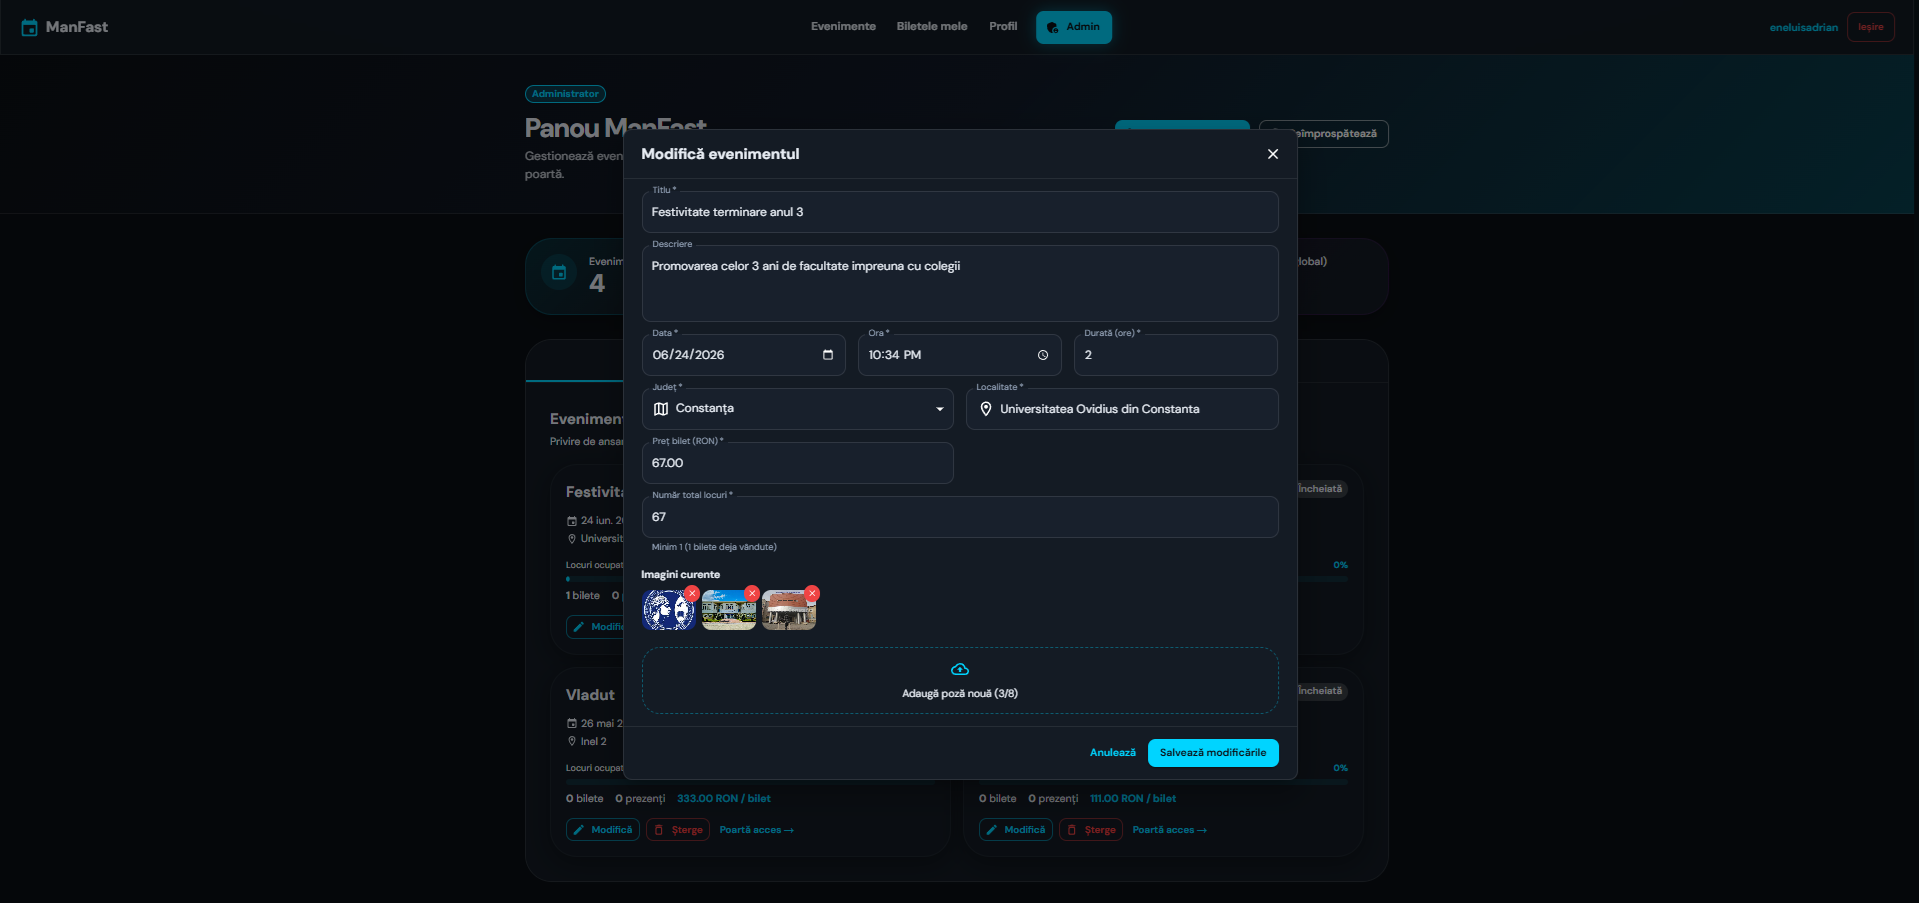
\includegraphics[width=1\textwidth]{Dialog editare eveniment.png}
	\caption{Dialog editare eveniment}
	\label{fig:l2f1}
\end{figure}

\subsection{Check-in participant}

Marcarea unui participant ca prezent (buton check-in sau toggle)

\begin{figure}[htbp]
	\centering
	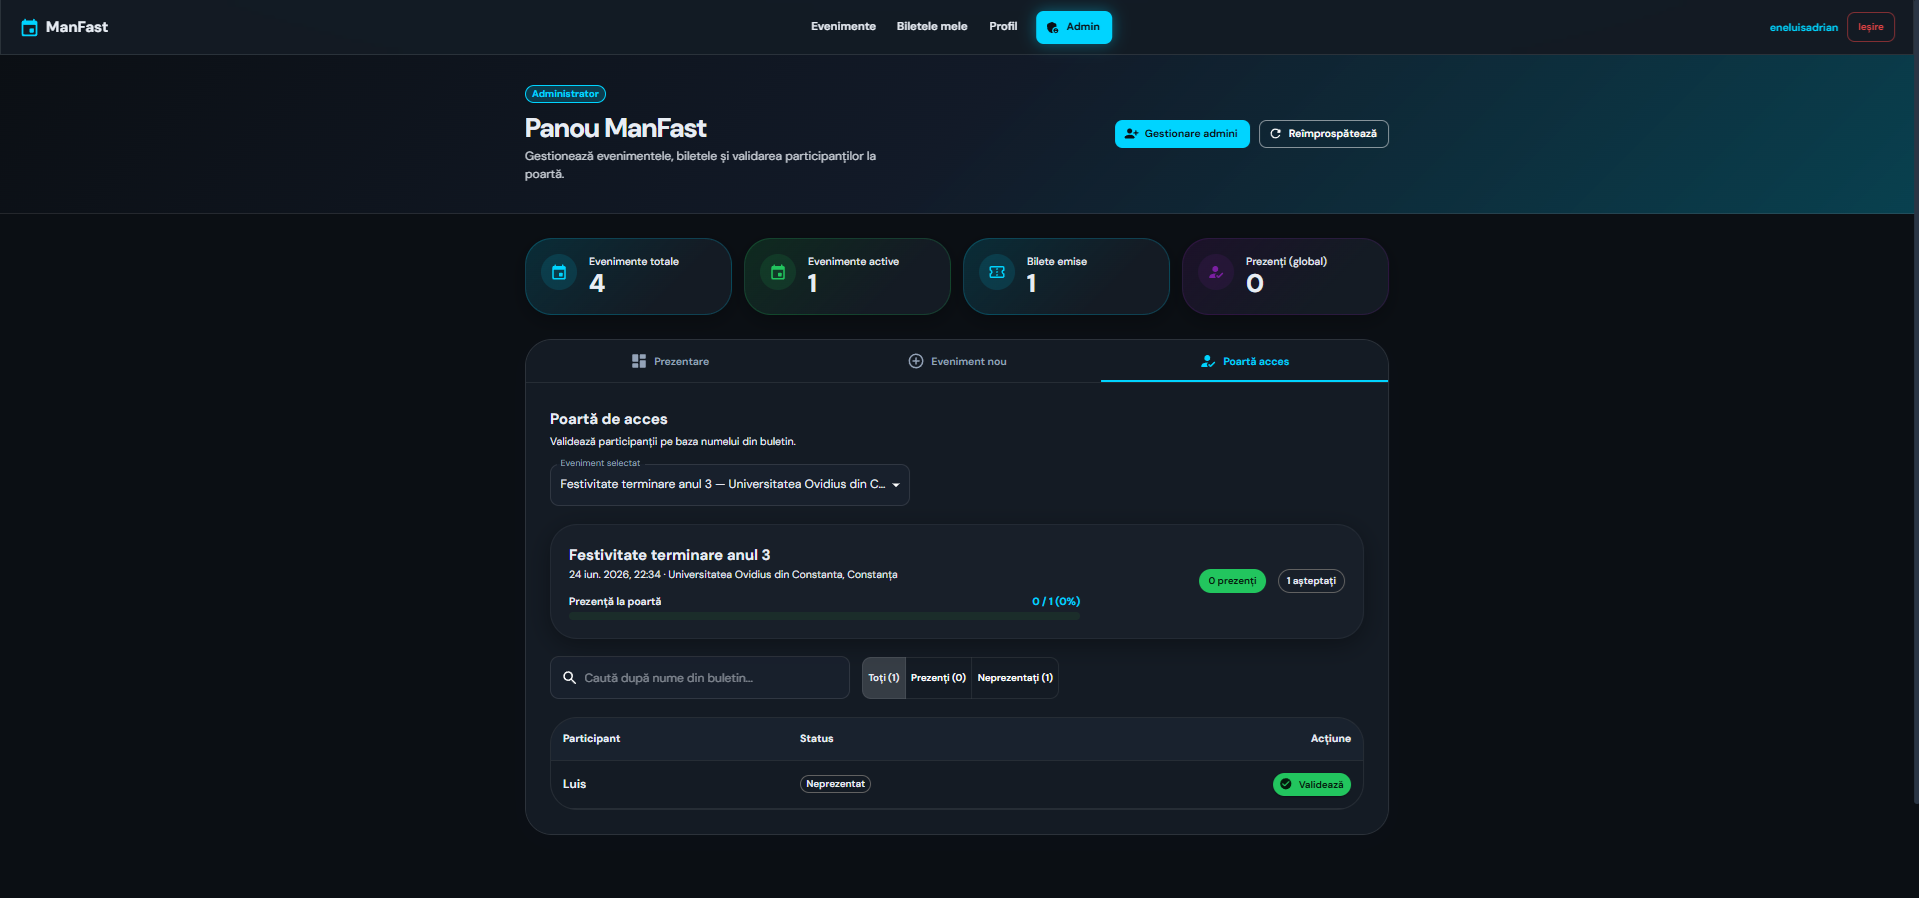
\includegraphics[width=1\textwidth]{Check-in participant.png}
	\caption{Check-in participant}
	\label{fig:l2f1}
\end{figure}

\begin{figure}[htbp]
	\centering
	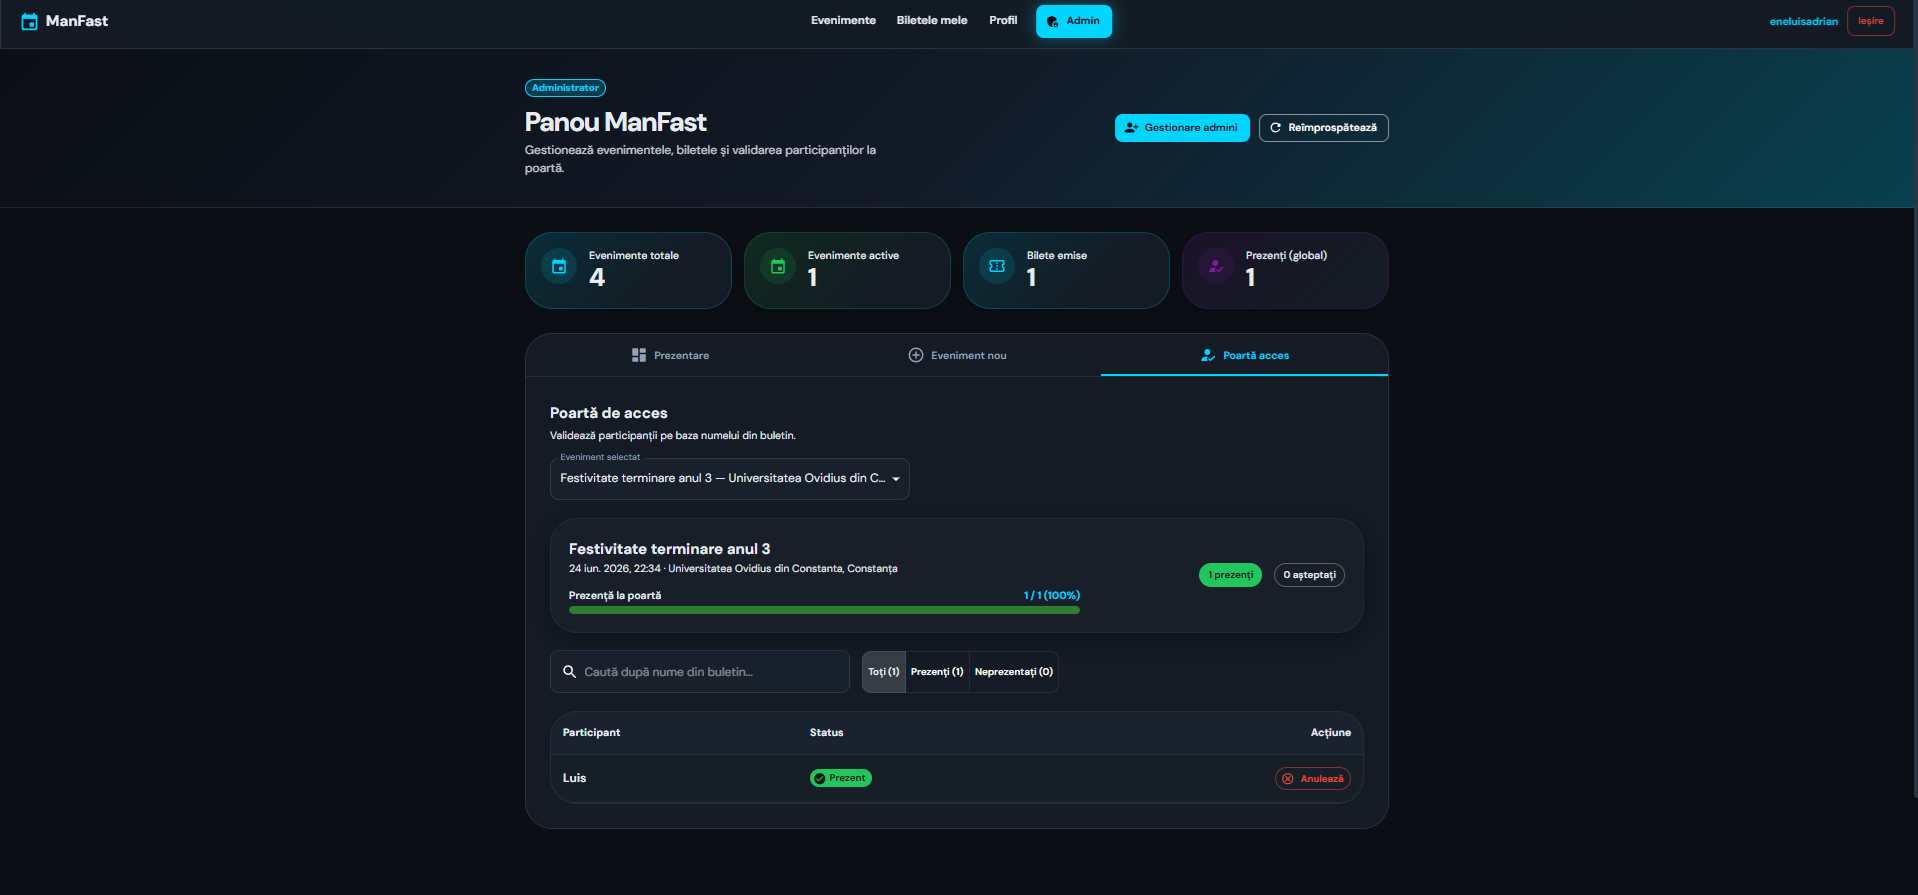
\includegraphics[width=1\textwidth]{Check-in participant2.png}
	\caption{Check-in participant validat}
	\label{fig:l2f1}
\end{figure}

\subsection{Gestionare administratori}

Dialog prmovare sau revocare admin cu parola autiorizare.

\begin{figure}[htbp]
	\centering
	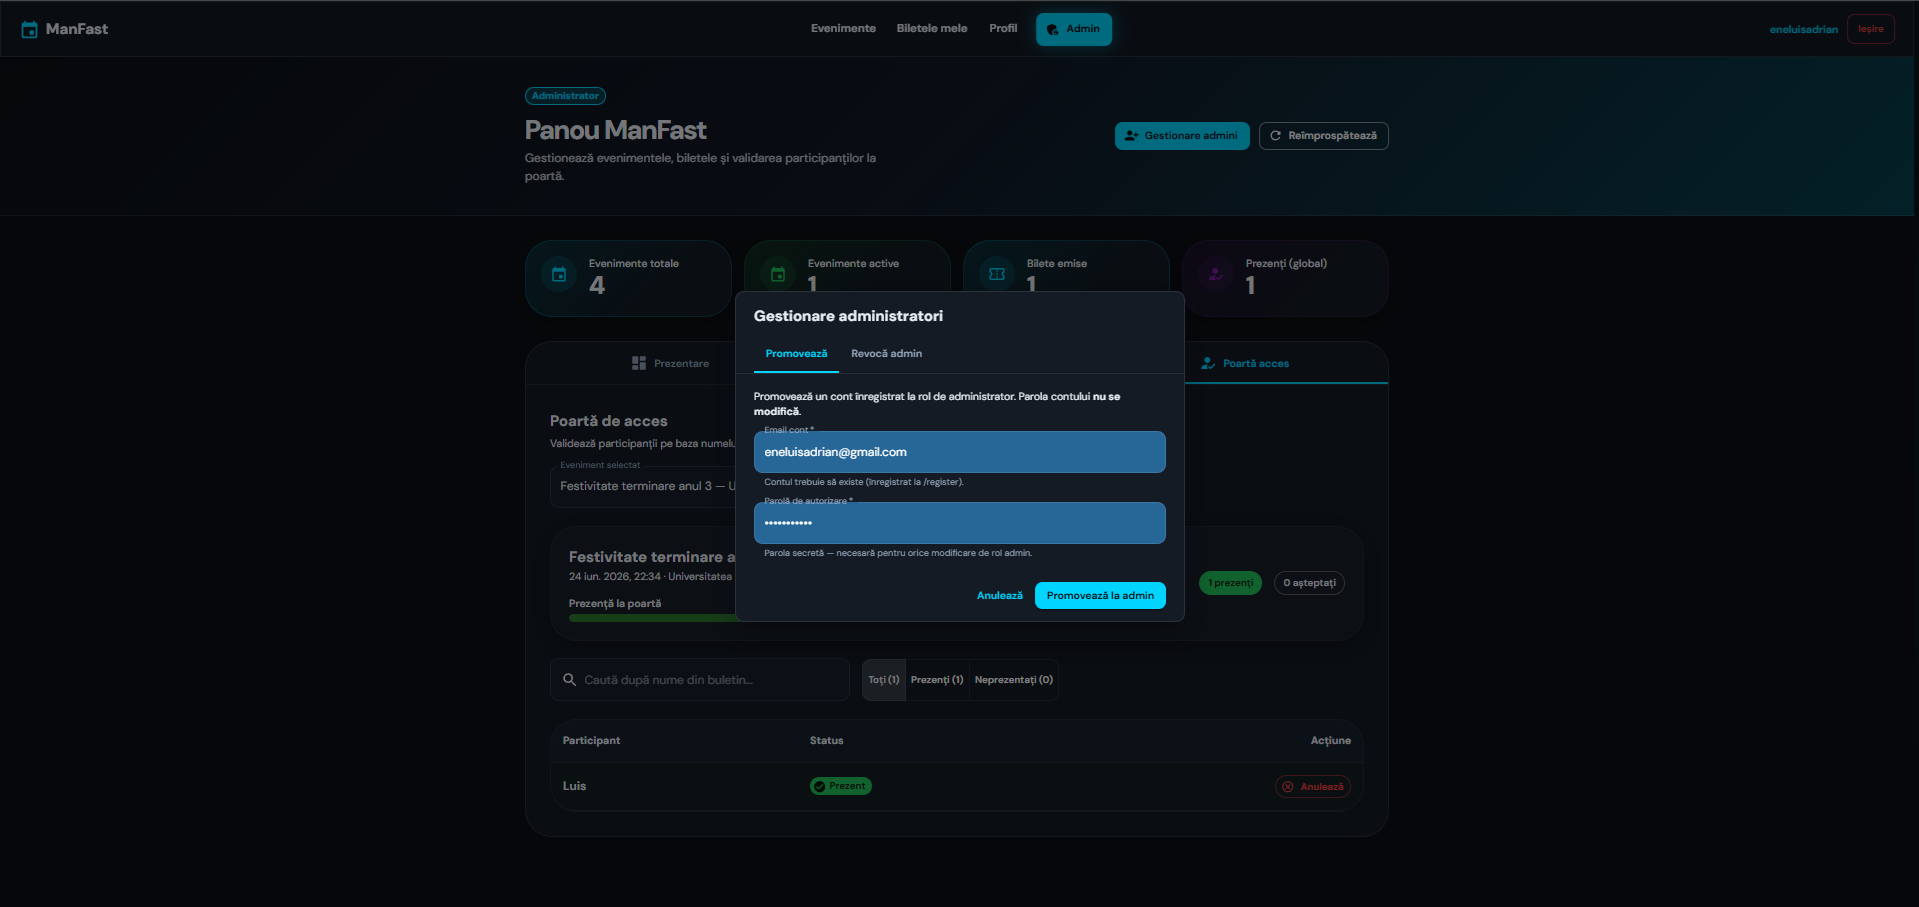
\includegraphics[width=1\textwidth]{Gestionare administratori.png}
	\caption{ Gestionare administratori}
	\label{fig:l2f1}
\end{figure}

\subsection{Conferință sau simpozion}

Pagina de detalii poate include în descriere: programul pe zile, lista speakerilor, link-uri către site-ul conferinței. Imaginile încărcate pot fi logo-ul evenimentului și fotografii din ediții anterioare. Filtrele de pe Home permit găsirea conferințelor dintr-un anumit județ sau dată — util pentru participanți care caută evenimente academice regionale.

Formularul de cumpărare bilet colectează numele participantului (pentru ecuson sau listă oficială). După plată, ,,Biletele mele`` afișează evenimentul ca ,,viitor`` până la data desfășurării; ulterior trece automat în ,,trecute``.

\subsection{Concert sau spectacol}

Organizatorul pune accent pe elementele vizuale: mai multe imagini (artiști, poster), descriere atractivă, preț și locuri limitate pentru a crea urgență. Utilizatorii pot cumpăra bilete pentru mai multe persoane introducând câte un nume per câmp — potrivit pentru ieșirile în grup.

Navbar-ul și tema dark oferă un aspect modern, aliniat la așteptările publicului tânăr pentru evenimente culturale. Pagina de succes după Stripe confirmă achiziția și redirecționează spre bilete.

\subsection{Meeting, workshop sau seminar}

Pentru evenimente profesionale cu număr mic de locuri, administratorul poate urmări în timp real câte locuri au rămas disponibile. Check-in-ul la intrare în sala de training confirmă prezența pentru certificat sau raport HR. Resetarea parolei și editarea profilului permit participanților să-și mențină contul pe termen lung, pentru evenimente recurente organizate de aceeași entitate.

\subsection{Eveniment sportiv (caz secundar)}

La competiții, numele de pe bilet poate corespunde actului de identitate al sportivului. Admin-ul bifează check-in la înregistrarea la concurs. Interfața nu afișează distincții specifice (categorie greutate, gen), dar fluxul tehnic este identic — organizatorul completează manual detaliile în titlu și descriere.

\subsection{Recomandări pentru capturi de ecran (capitol 4)}

Pentru o documentație reprezentativă, autorul poate crea în baza de date trei evenimente demonstrative:
\begin{itemize}
	\item ,,Conferința Națională Informatică 2026`` — accent pe descriere lungă și dată.
	\item ,,Concert Jazz Constanța`` — accent pe galerie imagini.
	\item ,,Workshop React pentru Începători`` — accent pe locuri limitate (ex. 25).
\end{itemize}

Capturile din figurile 4.1--4.8 pot folosi oricare dintre aceste evenimente; important este ca textul lucrării să reflecte diversitatea cazurilor, nu doar un singur domeniu.


\subsection{Accesibilitate și public larg}

Indiferent de categorie, formularele respectă etichetare clară, mesaje de eroare în română și layout responsive. Participanții mai puțin obișnuiți cu tehnologia (ex. invitați la conferință) beneficiază de flux liniar: Home $\rightarrow$ Detalii $\rightarrow$ Login/Register $\rightarrow$ Plată $\rightarrow$ Bilete.

Aceste exemple completează descrierea interfeței și leagă capturile de ecran de cazuri reale de utilizare în domeniul conferințelor, concertelor și meeting-urilor.